% !TeX root = ../main.tex
% Add the above to each chapter to make compiling the PDF easier in some editors.

\chapter{Explainability of News Content Models for Fake News Detection}\label{chapter:NewsContentModelsForFND}
The automated detection of fake news on social media comes with its characteristic challenges. The fact
that fake news pieces are constructed to misguide its consumers makes them hard to distinguish by only using news content. Fortunately, language models have become robust enough to capture patterns on different levels.\\
This chapter examines a language model, then inspects the model using explanation methods. In Section~\ref{sec:newsContentModels}, we lay out definitions and investigate the Transformer architecture. We analyze the dataset and report our findings. Then, we examine our news content classifier and share its performance on the dataset. Finally, in Section~\ref{sec:ExplainingNewsContentModels}, we outline the SHAP framework, which we later adopt to inspect the news content classifier's explainability.

\section{News Content Models}
\label{sec:newsContentModels}
A great share of FND methods utilizes news content. Models that base their predictions solely on news content focus on the patterns in the text, especially words or word groups that frequently appear in other instances of the same class. As discussed in Section~\ref{sec:fakeNewsDetection}, there exist a variety of approaches available for news content classifiers. However, many of the datasets discussed in the literature are unavailable or outdated. Therefore, we used a model that also provides its dataset.

\subsection{Notation and Definitions}
\label{subsec:newsContentModels_Definitions}
First and foremost, we introduce the notation used in this section in Table~\ref{tab:newsContentModels_Notation}.\\
\begin{table}
    \centering
    \def\arraystretch{1.5}
    \begin{tabular}{cp{0.8\textwidth}}
        $x^{raw} \in X^{raw}$ & A news article.                                              \\
        $y^{raw} \in Y^{raw}$ & A label of news article.                                     \\
        $T$                   & Tokenizer function                                           \\
        $\psi$                & Label mapping function                                       \\
        $x^{tok} \in X^{tok}$ & Tokenized news article                                       \\
        $y \in Y$             & Vectorized class value.                                      \\
        $|x^{tok}|$           & The number of tokens in $x^{tok}$.                           \\
        $\hat{y}$             & Prediction of model.                                         \\
        $x \in X$             & Numeric vector of $x^{tok}$                                  \\
        $|x|$                 & The length of input vector                                   \\
        $l$                   & Index of a layer                                             \\
        $a_{i}^{(l)}$         & The value of unit $i$ in layer $l$                           \\
        $w_{ij}^{(l)}$        & Weight between units $i$ in layer $l$ and $j$ in layer $l+1$ \\
        $\sigma$              & Activation function                                          \\
    \end{tabular}
    \caption[Notation]{Notation used in this section.}
    \label{tab:newsContentModels_Notation}
\end{table}
We define some relevant concepts utilizing the notation. First, we talk about terms and definitions for \emph{tokenization} and outline the tokenization process. First, to build upon a concrete foundation, let us consider a news article $x^{raw}$ fed to the tokenizer $T$.
\begin{definition}[\emph{Tokenizer}]
    A tokenizer $T:X^{raw} \mapsto X^{tok}$ is a function that maps raw textual data to smaller units called tokens.
\end{definition}
A token can be a word, character, or subword. Therefore, we define three types of tokenization techniques:
\begin{itemize}
    \item \emph{Word tokenization} splits the given text into individual words based on a delimiter, such as whitespaces or various punctuations. This approach creates a vocabulary from the inputs it was trained on. All words that do not appear in the vocabulary are replaced with an unknown token ([UNK]), and this concept is called being \emph{Out Of Vocabulary} (OOV). Depending on the task, the size of the vocabulary can grow quite large. The solution for exploding vocabulary sizes was introduced in subword tokenization. Commonly used examples of word tokenizers are Word2Vec~\parencite{Word2Vec_Mikolov} and GloVe~\parencite{GloVe_Pennington}.
    \item \emph{Character tokenization} splits the text into single characters. The number of available characters is limited, e.g., to 256; thus, there are no unknown words, which means there will be very few or no OOV words. However, the sequences can grow exponentially compared to word tokenization. For instance, the word "hello world" is two tokens long with whitespace word tokenization but eleven tokens long with character tokenization.
    \item \emph{Subword tokenization} splits the given text into subwords. For instance, comparative words like harder are segmented into "hard-" and "-er", or superlative words like hardest are segmented into "hard-" and "-est". The most common method for subword tokenization is \emph{Byte Pair Encoding} (BPE). BPE was introduced by~\cite{ANewAlgorithmForDataCompression_Gage} but adapted to word segmentation by~\cite{NeuralMachineTranslationOfRareWords_Sennrich}. BPE iteratively merges the most frequently appearing character or character sequences. This approach allows for efficient space usage and, thus, smaller vocabularies~\parencite{NeuralMachineTranslationOfRareWords_Sennrich}. This approach also helps the model learn similar words with the same roots.
\end{itemize}
We say that an input is \emph{tokenized} after it is fed to the tokenizer. A tokenized news article $x^{tok}$ is a vector of tokens in which the order of the words and characters in $x^{raw} \in X^{raw}$ are kept.
\begin{center}
    $T(x^{raw}) = x^{tok} = [x_1^{tok}, \dots, x_n^{tok}]$, where $n = |x^{tok}|$.
\end{center}
Usually, models accept a fixed size input. Hence, to get a fixed length output, the tokenized sequence $x^{tok}$ is padded with padding tokens ([PAD]) where the news article is not long enough. In case it is longer than the fixed length, then it is truncated. Some tokenizer implementations in Huggingface~\footnote{\url{https://huggingface.co/}} mask out the pads so that they are not included in the computation. These are called masked transformers~\parencite{Transformers_Wolf}. In fact, our news content classifier has the same behavior, which can be observed in~\ref{fig:InputTokenizationPipeline}.\\
\begin{figure}
    \centering
    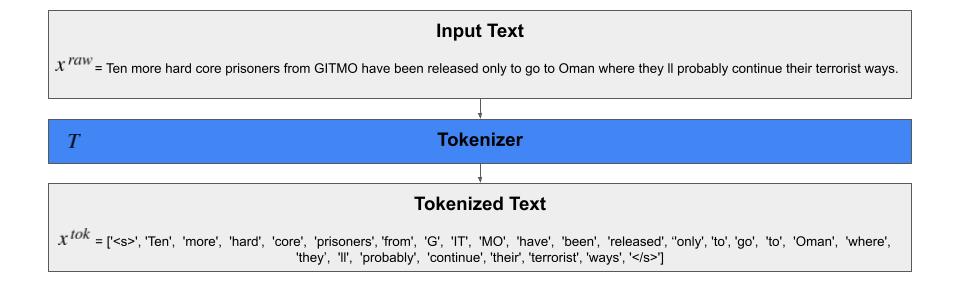
\includegraphics[scale=0.5]{InputTokenizationPipeline.png}
    \caption[The tokenization pipeline for a textual input.]{The tokenization pipeline for a textual input.}
    \label{fig:InputTokenizationPipeline}
\end{figure}
In order to feed the input to the model, we need numeric representation which can be obtained by various techniques. One widely used approach is the BoW representation which produces features based on the number of occurrences of a word or token. An alternative BoW representation uses the presence or absence of words in the vocabulary instead of frequencies. A more sophisticated approach is \emph{Word2Vec}, which encodes words into numeric values by learning word associations. From the perspective of the representation of a word, \emph{Word2Vec} can capture different degrees of similarity between words allowing for the preservation of semantic and syntactic relationships~\parencite{Word2Vec_Mikolov}. It is clear that the transformation of words into numeric vectors is a very crucial stage for FND since we need to maintain as much contextual information as possible. Nevertheless, the SOTA is an even more sophisticated approach called \emph{Transformer}, which is the building block of many powerful language models such as BERT.\\
We denote the space of raw label $Y^{raw} = \{"fake", "real"\}$, with $y^{raw} \in Y^{raw}$. We employ a label mapping function $\psi: Y^{raw} \mapsto Y$ that maps raw labels to classes, where $Y \in \mathbb{R}^2$ with,
\begin{center}
    \[\psi(y^{raw}) = y =
        \begin{cases}
            0, & if \;\; y^{raw} = "fake" \\
            1, & otherwise                \\
        \end{cases}
    \]
\end{center}
\begin{definition}[\emph{Classifier}]
    A classifier $f:X \mapsto Y$ is a function that outputs predicted scores $f(x)_y$ for each class $y$ for a given input $x$.
\end{definition}
Our classifier is a language model that was trained on a large corpus and a news dataset that contain fake and real news. It will predict whether a news piece is real or fake by assigning each label a probability.
\begin{definition}[\emph{Prediction}]
    A prediction $\hat{y}$ is the maximum of predicted scores $f(x)_y$ of a classifier.
    \begin{center}
        $\hat{y} = argmax_{y \in Y} f(x)_y$
    \end{center}
\end{definition}
We use a neural network classifier that consists of several layers and a complex architecture. Our model is able to work with large vocabularies and can classify news pieces based on various features.
\begin{definition}[\emph{Neural Network Classifier}]
    A neural network classifier is a \emph{classifier} $f$ that consists of layers $l$ with $1 \leq l \leq L$, where $L$ denotes the number of layers. Each layer has a set of units $a_i^{(l)}$, with $i$ denoting the position of the unit in layer $l$. We say that between two units, $a_i^{(l)}$ belonging to layer $l$ and $a_j^{(l+1)}$ belonging to layer
    $l+1$ have a weight value $w_{ij}^{(l)}$ that connects them. Along with a non-linear activation function $\sigma$, we
    can define the value of the $j$-th unit $a_j^{(l+1)}$ in terms of weights and unit values from the previous layer for an FCN, with $N$ as the number of units in layer $l$.
    \begin{center}
        $a_j^{(l+1)} = \sigma(\sum\limits_{i=1}^{N} a_i^{(l)} w_{ij}^{(l)})$
    \end{center}
\end{definition}
Neural networks are very powerful models. They can train millions of parameters using matrix multiplications, gradient-based optimization methods, and a fruitful set of other techniques, some of which will be discussed later. Neural networks iteratively optimize the weights between layers so that the produced output is as close to the desired output. This is achieved by using optimization methods, such as \emph{Gradient Descent} (GD)~\parencite{GD_Cauchy}, \emph{Stochastic Gradient Descent} (SGD)~\parencite{SGD_Robbins}, \emph{Adaptive Moment Estimation} (Adam)~\parencite{Adam_Kingma} that minimize the loss function defined for the problem. While many optimization methods are available for neural networks, we do not examine any of them.\\
\begin{figure}
    \centering
    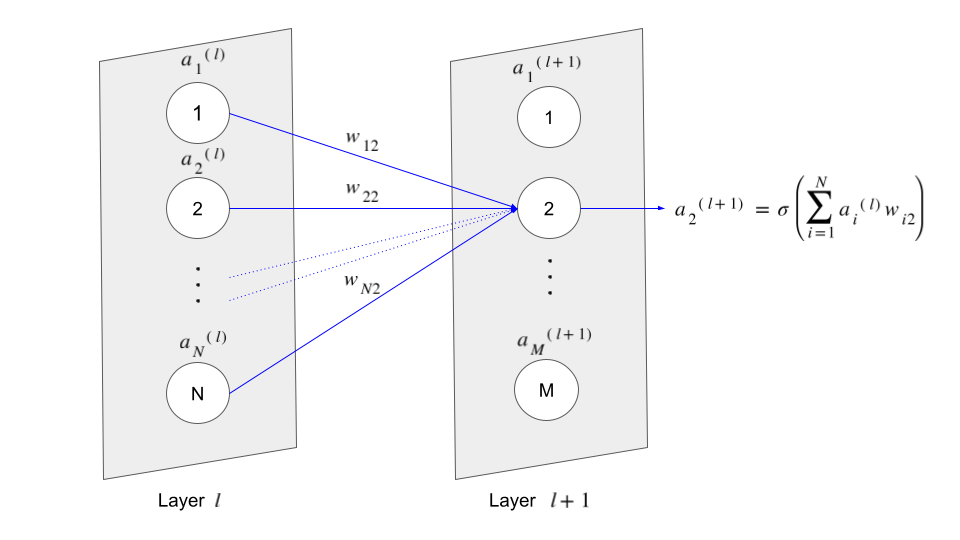
\includegraphics[scale=0.43]{NN_LayerRepresentation}
    \caption[Units and layers of an FCN.]{Units and layers of an FCN. For brevity, arrows and weights are only drawn for $a_2^{(l+1)}$.}
    \label{fig:NN_LayerRepresentation}
\end{figure}
For classification problems, we adopt a layer called \emph{Softmax}~\parencite{Softmax_Bridle} that outputs the predicted scores $f(x)_y$ for each class $y$ by normalizing outputs $Z_y(x)$ from the previous layer.\\
\begin{center}
    $f(x)_y = \dfrac{exp(Z_y(x))}{\sum\limits_{{y'} \in Y} exp(Z_{y'}(x))}$
\end{center}
The FCNs are the plainest architectures for neural networks. In an FCN, all units are connected. This means that there is a weight between each unit of the FCN and each unit of its previous layer. They are very straightforward to construct. Nevertheless, the usage of these architectures for modeling sequences is not preferred due to the exponential number of trained parameters. Instead, when modeling sequences like sentences and documents, a common approach is to adopt RNNs. RNNs allow previous outputs to be used while having hidden states. This permits information to pass through the sequence. However, vanilla RNNs are not powerful enough to represent long-term dependencies~\parencite{LearningLongTermDependenciesHard_Bengio} and suffer from vanishing/exploding gradients~\parencite{OnTheDifficultyOfTrainingRNNs_Pascanu}. \emph{Long Short-Term Memory} (LSTM)~\parencite{LSTM_Hochreiter} addresses the shortcomings of RNNs. The idea is to keep a cell state updated with the previous cell's state. This cell state is passed to the consequent cells to form a chain representing the document. More precisely, each cell corresponds to a token whose information will be shared with subsequent tokens by the propagation of cell states. This approach is indeed very useful for long documents since news articles tend to be long and their sentences contextually relevant. LSTM is usually used in different variations based on the same idea. For instance, a consequent study by~\citeauthor{LSTMPeephole_Gers} (\citeyear{LSTMPeephole_Gers}) has extended LSTMs with \emph{peephole connections}. LSTMs have been proven to deliver a good performance in NLP tasks such as \emph{speech recognition}~\parencite{AchievingHumanParityinConvSR_Wayne}. LSTMs perform well; however, they are being replaced with attention-based models due to long training times and large memory requirements during training.\\
One last thing to discuss is how the models are trained in terms of supervision. \emph{Supervised} models are trained with label data. \emph{Unsupervised} models work with unlabeled data and aim to find patterns in the data. An exciting setting is \emph{semi-supervised} models. These models are often provided with small amounts of labeled data and large amounts of unlabeled data for training. There are two settings for semi-supervised learning. \emph{Transductive} learning aims to predict unlabeled data, whereas \emph{inductive} learning samples unlabeled data from the same distribution to
infer the label~\parencite{LearningByTransduction_Gammerman}.\\
To summarize, we first outlined the process of a text becoming a numeric vector for a model. Then we discussed the classification steps and recapped the formation of neural networks. Finally, we argued about more capable model architectures employed in language models. Next, we will introduce the attention mechanism and Transformer models.

\subsection{Transformer Architecture}
\label{subsec:newsContentModels_TransformerArch}
Transductive learning has been successfully utilized along with the encoder-decoder structure in many language
tasks~\parencite{S2SLearningWithNNs_Sutskever, LearningPhraseRepresentations_Cho, AttentionIsAllYouNeed_Vaswani}. Transduction is first proposed by~\citeauthor{LearningByTransduction_Gammerman} (\citeyear{LearningByTransduction_Gammerman}) to counteract the unlabeled data problem. In contrast to supervised learning, transductive learning does not require all data to be labeled. Instead, it utilizes the clustered behavior of data. Transductive learning assigns labels to unlabeled data using the gaps between different clusters and a small set of labeled data. Transduction in sequence prediction is defined as a task where input sequences are transformed into output sequences~\parencite{SequenceTransdutionWithRNNs_Graves}. Transformer models are encoder-decoder structured language models that are designed for sequence transduction.\\
~\citeauthor{LearningPhraseRepresentations_Cho} (\citeyear{LearningPhraseRepresentations_Cho}) proposed an encoder-decoder structure that takes into account the order of words. This encoder-decoder structure consists of one RNN as the encoder and one RNN as the decoder. The encoder maps an input sequence to a fixed-length vector, and the decoder maps this fixed-length vector to a target sequence. Transformer architecture adopts a similar approach that employs feed-forward and Multi-Head Attention layers in both encoder and decoder, which is illustrated in Fig.~\ref{fig:transformerArchitecture} with N=6 stacks of encoders and decoders.\\
In order to reduce sequential computation, CNNs have been adopted as building blocks that parallelly compute hidden representations for all input and output positions~\parencite{AttentionIsAllYouNeed_Vaswani}. Although aimed to reduce computation, the number of operations to convey information from one random input or output to  the other increases linearly in ByteNet~\parencite{ByteNet_Kalchbrenner} and logarithmically in ConvS2S~\parencite{ConvS2S_Gehring}.\\
Contrary to CNNs, Transformers fix the number of operations by averaging attention-weighed positions, which decreases the effective resolution. However, this decrease in resolution is alleviated by using multi-head attention~\parencite{AttentionIsAllYouNeed_Vaswani}.
\begin{figure}
    \centering
    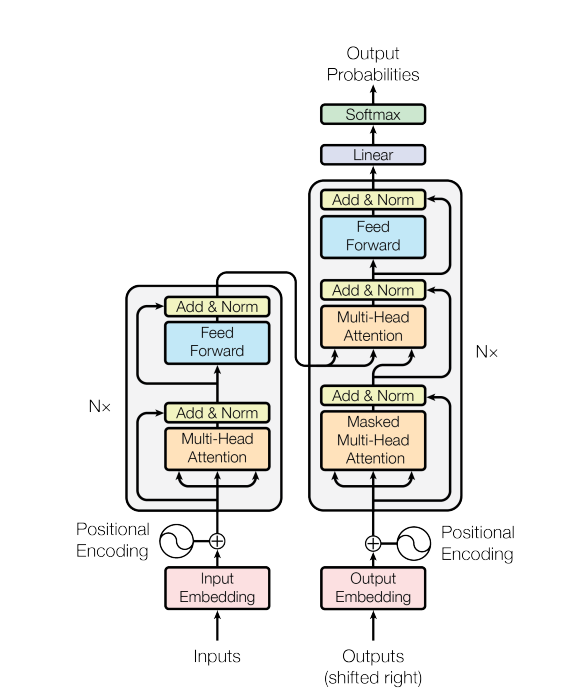
\includegraphics{TransformerArchitecture.png}
    \caption[The Transformer Model Architecture.]{The Transformer Model Architecture (N=6). Figure obtained from~\parencite{AttentionIsAllYouNeed_Vaswani}.}
    \label{fig:transformerArchitecture}
\end{figure}
Initially suggested in the decoder of the model proposed by~\citeauthor{NeuralMachineTranslationByJointlyLearning_Bahdanau} (\citeyear{NeuralMachineTranslationByJointlyLearning_Bahdanau}), an attention mechanism works similarly to human attention; it learns to put more importance on some words that convey the relevant information about the sentence. The attention mechanism that ~\citeauthor{NeuralMachineTranslationByJointlyLearning_Bahdanau} (\citeyear{NeuralMachineTranslationByJointlyLearning_Bahdanau}) use is called \emph{additive attention}. Inspired by additive attention,~\citeauthor{EffectiveApproachesToAttentionBased_Luong} (\citeyear{EffectiveApproachesToAttentionBased_Luong}) proposed a different approach called \emph{dot-product attention}, a form  that is also used in Transformer architecture.\\
% It does so by means of a context vector that depends on a sequence of \emph{annotations}. An annotation $h_i$ for a word (or token) $x_i$ contains information about the complete input sentence but with a focus on the words that are closer to the word $x_i$. The context vector $c_i$ for word $x_i$ is obtained as a weighted sum of all these annotations $h_i$~\parencite{NeuralMachineTranslationByJointlyLearning_Bahdanau}:
% \begin{center}
%     $c_i = \sum\limits_{j=1}^{|x|} \alpha_{ij} h_j$.
% \end{center}
% The weight $\alpha_{ij}$ is obtained by applying softmax to associated energy $e_{ij}$, which is an output of the alignment model $a$. The alignment model $a$ is a feed-forward neural network that jointly learns with the rest of the system. More precisely, we compute these values as follows~\parencite{NeuralMachineTranslationByJointlyLearning_Bahdanau}:
% \begin{center}
%     $\alpha_{ij} = \dfrac{e_{ij}}{\sum\limits_{k=1}^{|x|} exp(e_{ik})}$
% \end{center}
% where
% \begin{center}
%     $e_{ij} = a(s_{i-1}, h_j)$
% \end{center}
% with $s_i$ representing the current and $s_{i-1}$ the previous state of the
% model~\parencite{NeuralMachineTranslationByJointlyLearning_Bahdanau}. This is called \emph{additive attention}.\\
For Transformer models, the authors define the attention function as "\emph{mapping a query and a set of key-value pairs to an output, where the query, keys, values, and output are all vectors. The output is computed as a weighted sum of the values, where the weight assigned to each value is computed by a compatibility function of the query with the corresponding key.}"~\parencite{AttentionIsAllYouNeed_Vaswani}. The Transformer model employs two different attention mechanisms, namely, \emph{scaled dot-product attention} and \emph{multi-head attention}. Following~\parencite{AttentionIsAllYouNeed_Vaswani}, we denote that the input for the attention layers are matrices called queries $Q \in \mathbb{R}^{d_{model} \times d_k}$, keys $K \in \mathbb{R}^{d_{model} \times d_k}$, and values $V \in \mathbb{R}^{d_{model} \times d_v}$, with $d_k$ as the number of keys or values and $d_{model}$ being the model dimension. Scaled dot-product attention computes the dot product of all queries $q_i \in Q$ with all keys $K$ and scale the resulting weights with $\frac{1}{\sqrt{d_k}}$. After obtaining the softmax of the scaled weights, each weight is multiplied by the corresponding value to obtain attention values.
\begin{center}
    $Attention(Q, K, V) = softmax(\dfrac{QK^T}{\sqrt{d_k}})V$
\end{center}
The second attention mechanism, multi-head attention, uses multiple attentions, each of which uses a different learned linear projection of $Q$, $K$, $V$. Output of all of these attentions are then concatenated to obtain the final result. More precisely, it is computed as follows,
\begin{center}
    $MultiHead(Q, K, V) = Concat(head_1, head_2, \dots, head_h)W^{O}$
\end{center}
where each $head_i$ is calculated as,
\begin{center}
    $head_i = Attention(QW_i^Q, KW_i^K, VW_i^V)$
\end{center}
with projection for $Q$ as $W_i^Q \in \mathbb{R}^{d_{model} \times d_k}$, $K$ as $W_i^K \in \mathbb{R}^{d_{model} \times d_k}$, $Q$ as $W_i^V \in \mathbb{R}^{d_{model} \times d_v}$, and lastly, $W^{O} \in \mathbb{R}^{hd_v \times d_{model}}$~\parencite{AttentionIsAllYouNeed_Vaswani}.\\
We now outline each part of the Transformer model.\\
\begin{itemize}
    \item \emph{Encoder}: Consists of N=6 identical layers. Each of these layers has two sub-layers, the first of which uses multi-head attention and layer normalization~\parencite{LayerNorm_Ba} along with a residual connection~\parencite{ResidualConnection_He}. The second sub-layer consists of a feed-forward layer and layer normalization as well as a residual connection around the feed-forward layer~\parencite{AttentionIsAllYouNeed_Vaswani}
    \item \emph{Decoder}: Same as the encoder, this part is composed of N=6 layers. Additional to the previously discussed two sub-layers in the encoder, the decoder adopts a third sub-layer that computes the attention values over the output of the encoder. As it was done for the encoder, the decoder also utilizes layer normalization at the end of each sub-layer as well as the residual connection~\parencite{AttentionIsAllYouNeed_Vaswani}.
\end{itemize}
In the Transformer model, the embeddings are obtained through the embedding layer. All of the feed-forward networks in the sub-layers are position-wise, meaning that they are applied to each position separately and identically. These feed-forward networks use different parameters for each layer. Lastly, the positional encodings for input embeddings are calculated using sine and cosine functions of different frequencies~\parencite{AttentionIsAllYouNeed_Vaswani}. We will observe the effect of positional encodings when explaining the news content classifier.\\
In order to lay the foundations for the model we adopted, we have introduced its structure and mechanism. Next, we initially introduce details of BERT, then RoBERTa, and lastly DistilRoBERTa which is the base of our choice of news content classifier.

\subsection{Dataset and Model}
\label{subsec:newContentModel_DatasetAndModel}
We employ a fine-tuned version of the case-sensitive Transformer model DistilRoBERTa\footnote{\url{https://huggingface.co/GonzaloA/distilroberta-base-finetuned-fakeNews}} for our task of FND with news content. DistilRoBERTa is a distilled version of \emph{A Robustly Optimized BERT Pretraining Approach} (RoBERTa)~\parencite{RoBERTa_Liu}. It uses the same distillation procedure adopted to build  DistilBERT~\parencite{DistilBERT_Sanh} using \emph{Bidirectional Encoder Representations from Transformers} (BERT)~\parencite{BERT_Devlin}. This distillation procedure is referred to as \emph{knowledge distillation} and it compresses a model~\parencite{ModelCompression_Bucilua} - the teacher - by means of training a smaller model - the student - to reproduce the same behavior~\parencite{DistillingTheKnowledge_Hinton}. In our case, the teacher is  RoBERTa and the student is DistilRoBERTa. First, in order to examine the properties of RoBERTa, we discuss BERT in detail.\\
As the name suggests, the model architecture of BERT is a multi-layer bidirectional Transformer model. BERT uses BookCorpus~\parencite{BookCorpus_Yukun} and English Wikipedia as training datasets, with two training objectives, \emph{Masked Language Modeling} (MLM) and \emph{Next Sentence Prediction} (NSP).\\
NSP procedure is a binary classification loss that predicts whether two segments (sequences of tokens) are consecutive in
the original text. \emph{Positive} and \emph{negative} examples are sampled with equal probability in this process.
Positive examples are created by taking consecutive sentences from the text corpus, whereas negative examples
are generated by pairing segments from different documents~\parencite{BERT_Devlin,RoBERTa_Liu}.\\
MLM procedure applies the following for each sentence sampled from a document in the cumulative dataset.
\begin{itemize}
    \item Mask 15\% of the tokens.
    \item In 80\% of the cases, replace the masked tokens with [MASK].
    \item In 10\% of the cases, replace the masked tokens with a different random vocabulary token.
    \item In the remaining 10\% of the cases, the masked tokens are left unchanged.
\end{itemize}
RoBERTa is an optimized version of BERT. It was pretrained longer using longer sequences. RoBERTa uses MLM as the training objective but not NSP. Contrary to BERT, RoBERTa keeps a dynamic masking pattern that changes in training. It is
pretrained on the reunion of five datasets (three more datasets than BERT) that size up to 160 gigabytes (GB): BookCorpus~\parencite{BookCorpus_Yukun},
English Wikipedia~\parencite{EnglishWikipedia_Wiki},
CC-News~\parencite{CCNews_Nagel}, OpenWebText~\parencite{OpenWebText_Radford},
Stories~\parencite{ASimpleMethodForCommonsenseReasoning_Trinh}.\\
RoBERTa tokenizes texts using BPE with a vocabulary size of 50,000 and maximum sequence length (maximum number of tokens) as 512. The beginning and end of each document (news article) is marked with <s> and </s>, respectively. With MLM as the training objective and Adam~\parencite*{Adam_Kingma} as the optimizer, the model reaches better results than BERT. Additionally, it should be noted that these models are further trained for downstream tasks; thus, we refer to the training stage as pretraining to avoid any confusion.\\
DistilRoBERTa has the same general architecture as RoBERTa, but the number of layers is reduced by a factor of two, and the
\emph{token-type embeddings} and the pooler are removed. Then DistilRoBERTa is initialized with layers from the teacher.
The distillation is done with very large batches~\parencite{DistilBERT_Sanh}. Using RoBERTa as a teacher, the student DistilRoBERTa is pretrained on OpenWebTextCorpus~\parencite{OpenWebTextCorpus_Gokaslan}, a reproduction of OpenWebText~\parencite{OpenWebText_Radford}.\\
The model we employed from Huggingface used a dataset curated from different sources for training~\footnote{\url{https://huggingface.co/datasets/GonzaloA/fake_news}}. To clarify, this model was already trained, i.e., we did not train this model. Although there exist better datasets and news content classifiers, we opted for this particular model for two reasons. First, most SOTA news content classifiers do not provide their code and dataset to reproduce results. Second, since Transformers are SOTA and this particular trained model provides us with not only the dataset but also the train/test/validation splits, which allows us to analyze its explanation.\\
\textbf{Dataset.} The news content dataset comprises 40587 samples whose distribution of labels and train/validation/test splits are provided in Fig~\ref{fig:DatasetDistributionByLabelAndSplit}. The proportion of fake news is 46\%, which is a fair distribution between real and fake news instances. The train/validation/test split is the common practice 60\%/20\%/20\%.
\begin{figure}
    \centering
    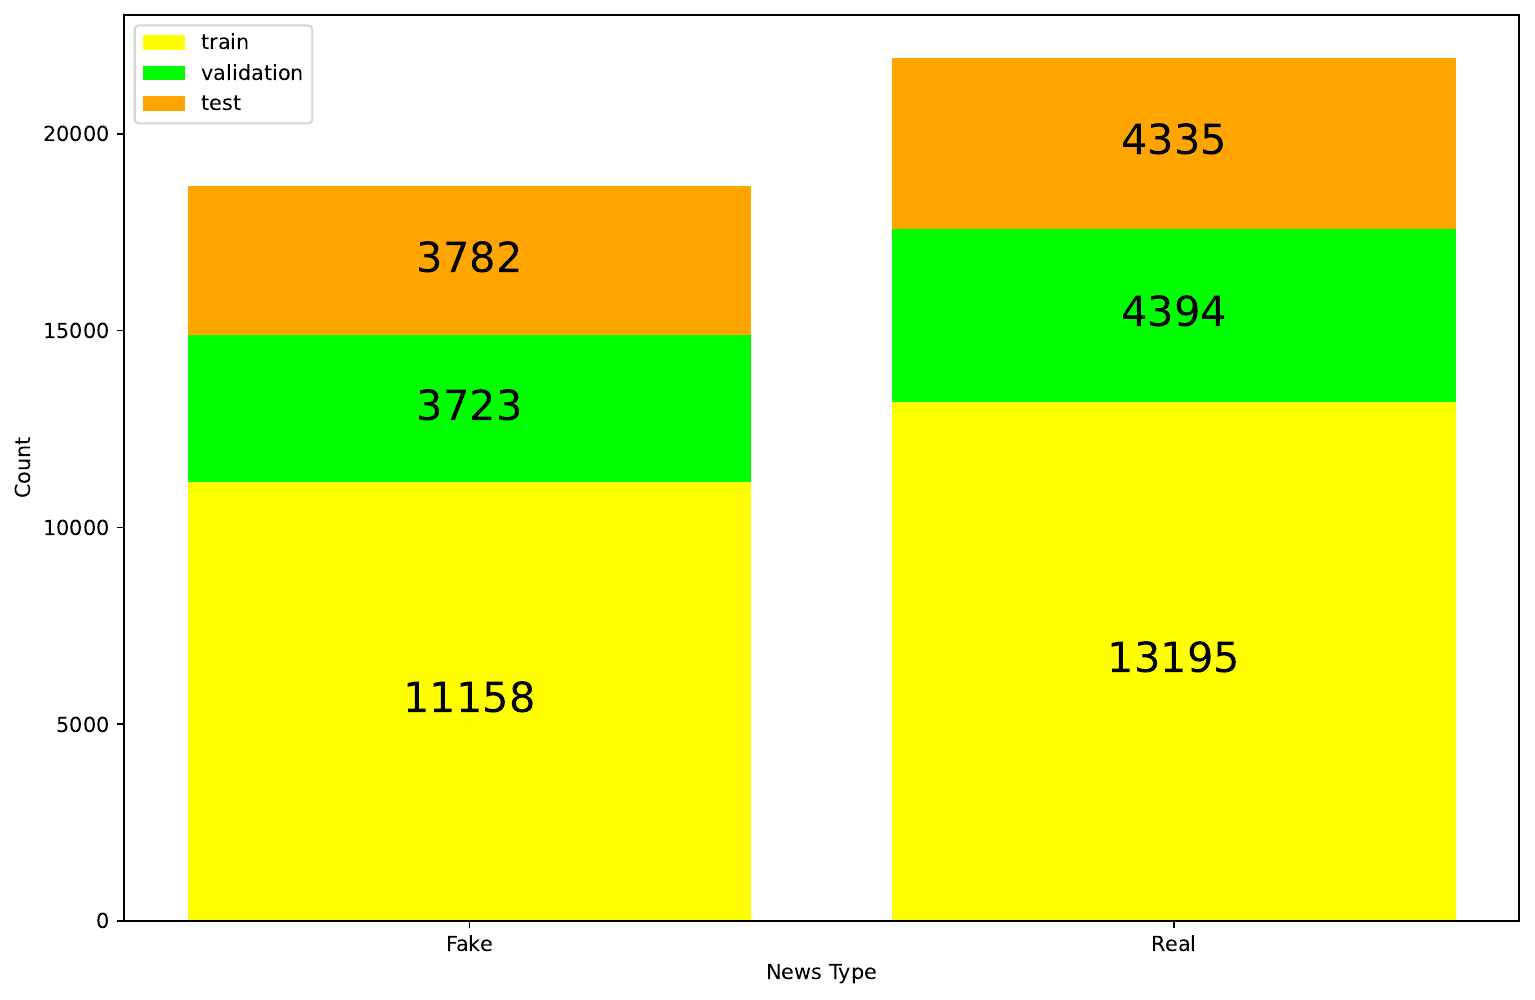
\includegraphics[scale=0.5]{DatasetDistrByLabelAndSplit.png}
    \caption[News content dataset distribution by label and train/validation/test split.]{News content dataset distribution by label and train/validation/test split.}
    \label{fig:DatasetDistributionByLabelAndSplit}
\end{figure}
We analyze the 500 most frequently occurring tokens in the dataset using a WordCloud~\parencite{WordCloud_Oesper} visualization for all samples of real and fake news separately in Fig~\ref{fig:WordCloudVisualizations}. From the visualization, we can observe that samples from both datasets contain the words "new", "state", "President", "Republican". In fact, the 500 most frequent tokens from fake news samples and real news samples share 63\% of tokens. Furthermore, we observe that one of the most frequent tokens is "Reuters" in real news instances. In fact, 95.93\% of real news samples contain the token coalition "(Reuters)". It is crucial to note that the idea of analyzing the frequency of keywords was initially formed once we started explaining the news content classifier. We will share how we draw this insight in the following section.\\
\begin{figure}
    \centering
    \subfloat[Fake news]{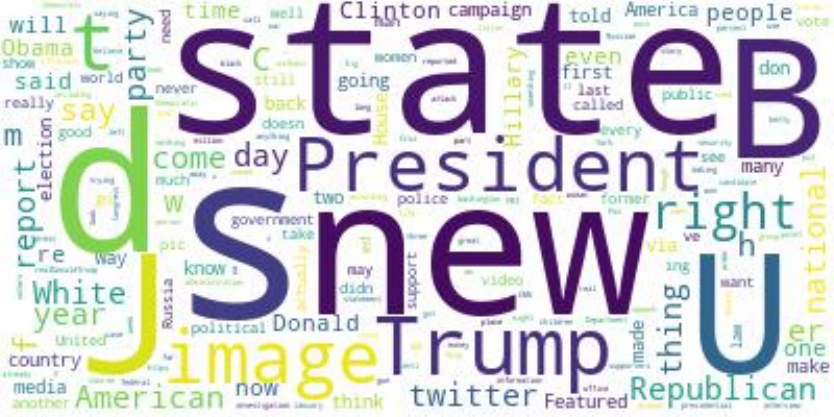
\includegraphics[width=0.45\textwidth]{DatasetFakeFrequentTokensWordCloud.png}\label{subfig:WordCloud_DatasetFakeFrequentTokensWordCloud}}
    \hfill
    \subfloat[Real news]{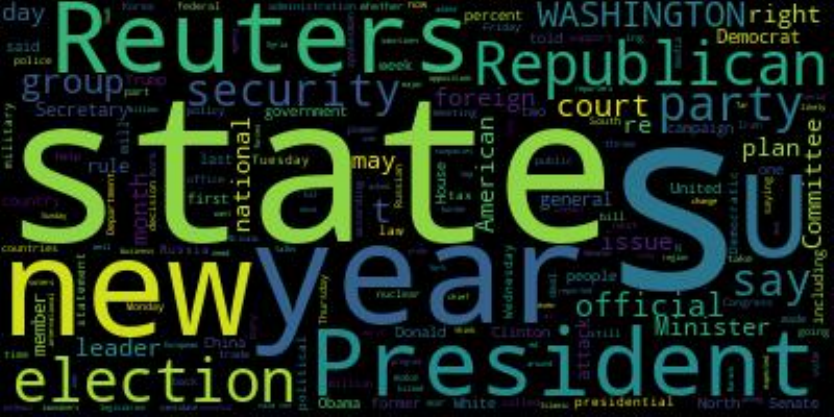
\includegraphics[width=0.45\textwidth]{DatasetRealFrequentTokensWordCloud.png}\label{subfig:WordCloud_DatasetRealFrequentTokensWordCloud}}
    \caption[WordCloud visualiations for most frequently occurring 500 tokens in both classes.]{WordCloud visualiations for most frequently occurring 500 tokens in samples of both classes.}
    \label{fig:WordCloudVisualizations}
\end{figure}\\
\textbf{Training.} Huggingface provides us with a \emph{TextClassificationPipeline} which allows feeding the dataset from Huggingface directly~\parencite{Transformers_Wolf}. This pipeline includes the tokenization process, DistilRoBERTa, and a classification layer. Our news content classifier has six layers, 12 attention heads, and a hidden size of 768 that totals up to 82M parameters (RoBERTa has 125M parameters). The vocabulary size is 50265, including special tokens. The model also uses a technique called \emph{dropout} which is a regularization technique that drops some connections between units of layers based on a probability value~\parencite{Dropout_Nitish}. All model hyperparameters are defined in~\ref{tab:newsContentModelHyperparameters}.\\
\begin{table}
    \centering
    \begin{tabular}{|l|l|}
        \hline
        Attention dropout probability           & 0.1                             \\
        \hline
        Batch size                              & 16                              \\
        \hline
        Epochs                                  & 3                               \\
        \hline
        Hidden layer activation function        & GELU~\parencite{GELU_Hendrycks} \\
        \hline
        Layer normalization factor ($\epsilon$) & 1e-05                           \\
        \hline
        Learning rate                           & 2e-05                           \\
        \hline
        Maximum position embeddings             & 514                             \\
        \hline
        Number of attention heads               & 12                              \\
        \hline
        Number of layers                        & 6                               \\
        \hline
        Vocabulary size                         & 50265                           \\
        \hline
        Weight Decay                            & 0.01                            \\
        \hline
    \end{tabular}
    \caption[Hyperparameters of the news content classifier.]{Hyperparameters of the news content classifier.}
    \label{tab:newsContentModelHyperparameters}
\end{table}
Note that the maximum position embeddings parameter also considers document start and end tokens when reporting its length. When feeding tokens $x^{tok}$ to the model, the start (<s>) and end (</s>) tokens are added by the model pipeline, so this leaves us with a maximum sequence length of 512, i.e., $|x|=512$. Note that in Figure~\ref{fig:InputTokenizationPipeline}, the length of $x$ is not 512 since the paddings are masked out in the attention mask before feeding the input $x$ to the model. We only illustrated values for tokens that exist, as pads will receive a value that has no effect on the calculation of the output, such as 0. \\
\textbf{Performance Evaluation.} The model is trained for three epochs with a batch size of 16, and Adam ($\beta_1=0.9$, $\beta_2=0.999$, $\epsilon=1e-08$) as the optimizer. The performance metrics for the model are provided in Table~\ref{tab:newsContentModelPerformanceMetrics}. To evaluate, the model performs very well on the dataset. Only 93 samples out of 8117 are classified incorrectly in the test split. Out of that 93 samples, 51 of them are fake news instances, and the rest are real news instances. However, good performance does not necessarily suggest that the model has learned its task. It might have found a simple pattern between fake and real news instances and based its prediction on this trivial feature. This is why explaining a model is crucial. We can inspect the news content classifier's behavior under different cases using explanation techniques.\\
\begin{table}
    \centering
    \begin{tabular}{c | c | c | c}
        \textbf{Accuracy} & \textbf{Precision} & \textbf{Recall} & \textbf{F1 score} \\
        \hline
        98.85\%           & 98.82\%            & 99.03\%         & 98.92\%           \\
    \end{tabular}
    \caption[The performance metrics for news content classifier.]{The performance metrics for news content classifier.}
    \label{tab:newsContentModelPerformanceMetrics}
\end{table}
We have laid out the foundations for the model we used to understand the news content model's learning mechanism. We reported the characteristics, training details, and performance of the news content classifier in this section. Our news content classifier seems to have learned its task very well. However, if this model was to be deployed for FND, then we need to see its performance in different settings, such as against adversarial approaches. We will explain the news content classifier by adopting methods from the coalitional game theory.

\section{Explaining News Content Models}
\label{sec:ExplainingNewsContentModels}
Although there exist models that can detect fake news with high accuracies, such as the news content classifier we adopted, the reasons behind this performance are seldom investigated. There could be a number of reasons, from dataset characteristics to wrong model architecture. Just by looking at a model's performance on a single dataset, one should not trust the model's spectacular performancee. Instead, look at the reasons to understand why this is happening. Is the model actually learning to distinguish between classes, or is it learning some other thing that we do not want? The explanation of this model can also tell the model's type in terms of style-based FND approaches. Does the news content classifier capture features based on objectivity or deception? In order to answer questions like these and more,~\citeauthor{AUnifiedApproach_Lundberg} (\citeyear{AUnifiedApproach_Lundberg}) propose a unified framework in which any model (except GNNs) can be explained.\\
We start this section by describing how the Shapley Additive exPlanation (SHAP) framework helps explain a model. After examining the SHAP framework, we utilize it for the news content classifier and examine the reasons behind its performance by conducting several experiments.\\
\subsection{The SHAP Framework}
\label{subsec:ExplainingNewsContentModels_SHAPFramework}
The SHAP framework aims to explain a prediction of a single input instance $x$ by computing Shapley values from coalitional game theory. These values correspond to the contribution of each input feature to the prediction made for $x$~\parencite{InterpretableMachineLearning_Molnar}. Specifically, we are interested in SHAP's ability to capture local explanations
for our news content classifier. Fortunately, SHAP provides explanation frameworks for a variety of models, including DNNs. In order to handle DNNs, SHAP improves methods from DeepLIFT to produce DeepSHAP. However, DeepSHAP is not compatible with Transformer models. Thus, we use a model-agnostic explanation model provided in the SHAP framework, namely the partition explainer. We begin with introducing Shapley values which are then converted to Owen values via feature coalitions. We will examine how Owen values and Shapley values are connected.\\
As before, let us denote our news content classifier to be explained as $f$ and its input as $x$. We focus on local explanations built for a single prediction $\hat{y} = f(x)$ based on one input $x$. An explanation model $g$ employs a simplified input $x'$, which is the output of a mapping function $h_x(x') = x$ that maps $x$ to $x'$. Each $h_x(x')$ is defined individually for each $x$. If two simplified inputs are similar $x' \sim z'$ then local methods aim to guarantee the approximation $g(z') \approx f(h_x(z'))$~\parencite{AUnifiedApproach_Lundberg}.\\
The general framework is built upon \emph{additive feature attribution methods}. These methods \emph{have an explanation model that is linear of binary variables}~\parencite{AUnifiedApproach_Lundberg}.\\
\begin{center}
    $g(z') = \phi_0 + \sum\limits_{i=1}^M \phi_i z_i'$
\end{center}
where $z' \in \{0, 1\}^M$, $M$ denotes the number of simplified input features, and $\phi_i \in \mathbb{R}$ feature relevance score of feature $i$~\parencite{AUnifiedApproach_Lundberg}. Note that $\phi_0$ corresponds to the base value, and can be used as an indicator to detect the bias in a model. Additive feature attribution methods have three desired properties. The first, local accuracy, states that \emph{the explanation model} $g(x')$ \emph{matches the original model} $f(x)$ \emph{when} $x = h_x(x')$~\parencite{AUnifiedApproach_Lundberg}. The second property is missingness, and it states that the features not included in the input should have no impact~\parencite{AUnifiedApproach_Lundberg}. The last property, consistency describes that if a simplified feature $x_i' \in x'$ have a greater impact in model $f'$ than the model $f$, then the feature $x_i$ should be assigned at least the same or a higher value for its contribution~\parencite{AUnifiedApproach_Lundberg}. \\
The computation of each $\phi_i$ involves a similar process to the calculation of classic Shapley regression values~\parencite{AnalysisOfRegressionInGameTheory_Lipovetsky}:
\begin{center}
    $\phi_i(f, x ) = \sum\limits_{z' \subseteq x'} \dfrac{|z'|! (M - |z'| - 1)!}{M!} [f_x(z') - f_x(z' \setminus i)]$
\end{center}
where $z' \setminus i$ implies $z_i' = 0$, $|z'|$ is the number of non-zero elements in $z'$, and $z' \subseteq x'$ denotes the set of vectors $z'$ whose non-zero elements are a subset of non-zero elements in $x'$~\parencite{AUnifiedApproach_Lundberg}.\\
% In the supplementary material of~\cite{AUnifiedApproach_Lundberg}, the authors define four axioms all of which Shapley values satisfy.
% \begin{enumerate}
%     \item \emph{Efficiency forces the model to correctly capture the original predicted value}~\parencite{AUnifiedApproach_Lundberg}
%     \item \emph{Symmetry states that if two features contribute equally to the model then their effects must be the same}~\parencite{AUnifiedApproach_Lundberg}.
%     \item \emph{Null effects} denotes that if a feature is missing in all subsets and this feature does not affect the outcome of the model, then this feature is ignored and its effect must be 0~\parencite{AUnifiedApproach_Lundberg}.
%     \item \emph{Linearity} states that if two models are written as a linear combination, then the sum of the effect of a feature in both models represent the effect of feature in the linear combination~\parencite{AUnifiedApproach_Lundberg}.
% \end{enumerate}
% Symmetry, null effects, and linearity are proven to be satisfied with the monotonocity axiom by~\citeauthor{MonotonicSolutionsOfCooperativeGames_Young} (\citeyear{MonotonicSolutionsOfCooperativeGames_Young}) and~\citeauthor{AUnifiedApproach_Lundberg} (\citeyear{AUnifiedApproach_Lundberg}). Therefore, we only need monotonocity and efficiency to be satisfied to constrain ourselves to using Shapley values. Owen values satisfy these constraints. 
Given a hierarchy of features that define feature coalitions, the partition explainer recursively computes Shapley values through them, and these Shapley values result in Owen values~\parencite{OwenValues_Owen}. Owen values are not the same as Shapley values, but if the coalition consists of the whole sentence or individual tokens, then Owen values and Shapley values become equal. A study~\parencite{TheOwenAndShapleyValue_Casajus} also shows that Shapley values are the expected Owen values for all symmetric distributions on all partitions. Owen values will help us detect token groups (if any exist) that play a significant role in the prediction of a model. Moreover, Owen values are computationally very cheap which, makes them more attractive.\\
We have summarized the foundations of the SHAP framework. As recommended in the source code documentation of SHAP\footnote{\url{https://github.com/slundberg/shap/}}, we use the partition explainer for our Transformer language model. Next, we will examine Owen values in action with our news content classifier.

\subsection{Explainability of The News Content Classifier}
\label{subsec:ExplainingNewsContentModels_ExplainingNewsContentClassifier}
Having introduced the required concepts, we now utilize them to explain the news content classifier using some real and fake news instances from the dataset. We adopt the partition explainer in order to understand how our Transformer model works. We specifically try to find its shortcomings so that we can decide whether it is a good idea to use this FND system in real cases.\\
\textbf{Initial Analysis.} We took a fake news example from the train split of the dataset and analyzed which tokens are deemed most important. The explanation provided by the partition explainer for our first fake news instance is illustrated in Fig.~\ref{fig:FakeNewsExample1_forceplot}. We can quickly observe that the base value is too high. In a normal setting, the base value should be around $0.5$ for a binary classifier. Apart from a high base value, the model is actually capturing sensible features. For example, it can detect a non-formal narrative using words like "ride", "hood", "The genius protestors".  Interestingly, punctuations such as ".", "," and ". "were given particularly high importance even though they should not contribute to the context of the news that much.\\
\begin{figure}
    \centering
    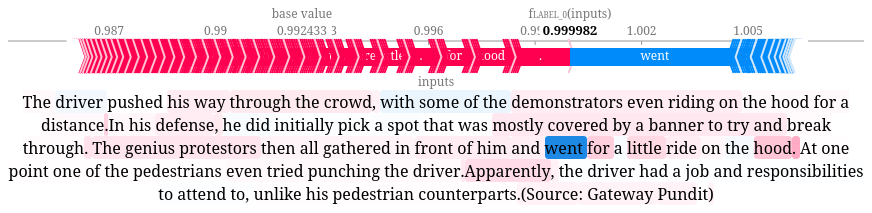
\includegraphics[scale=0.45]{FakeNewsExample1_forceplot.png}
    \caption[The explanation provided by SHAP partition explainer for our first fake news example.]{The explanation provided by SHAP partition explainer for our first fake news example. Example obtained by randomly selecting from our train split.}
    \label{fig:FakeNewsExample1_forceplot}
\end{figure}
% \begin{figure}
%     \centering
%     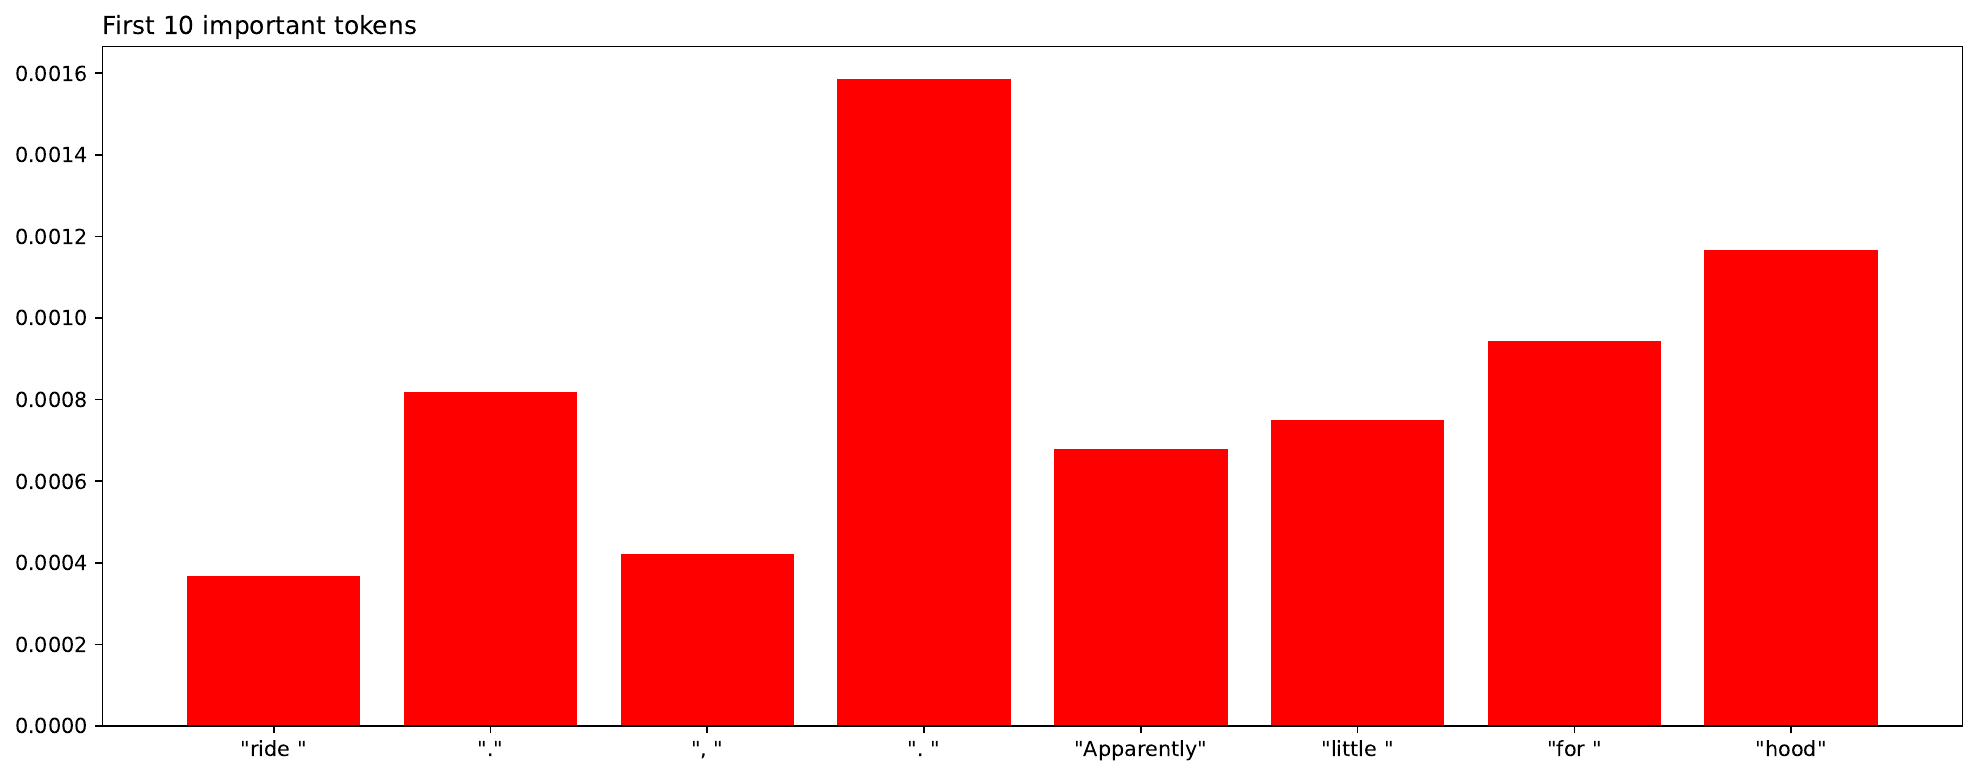
\includegraphics[scale=0.33]{FakeNewsExample1_barplot.png}
%     \caption[The barplot of the 10 highest Owen values and their tokens for the first fake news example.]{The barplot of the 10 highest Owen values and their tokens for the first fake news example. Since the news articles are long texts, we used a bar plot to visualize important tokens' Owen values.}
%     \label{fig:FakeNewsExample1_barplot}
% \end{figure}
We explain one more fake news instance from train split to see if the model behaves the same for that instance as well. The example is illustrated in Fig~\ref{fig:FakeNewsExample2_forceplot}. We can quickly observe that the model was able to capture non-formal speech again. We further examine how the tokens and coalitions are constructed. We see that "not a U." and "S. citizen." are separate coalitions. This implies that the tokenizer evaluated "U." and "S." as separate tokens. This issue might have occurred due to the punctuations between "U" and "S". Typically, one would expect "U.S." to be tokenized as one token, but the tokenizer failed to capture this. Following this issue, we realized that the tokenizer splits capitalized words into smaller units, which suggests the tokenizer is not capable of understanding most capitalized words. This might not be good for the news content classifier. In addition, the base value is again too high.\\
\begin{figure}
    \centering
    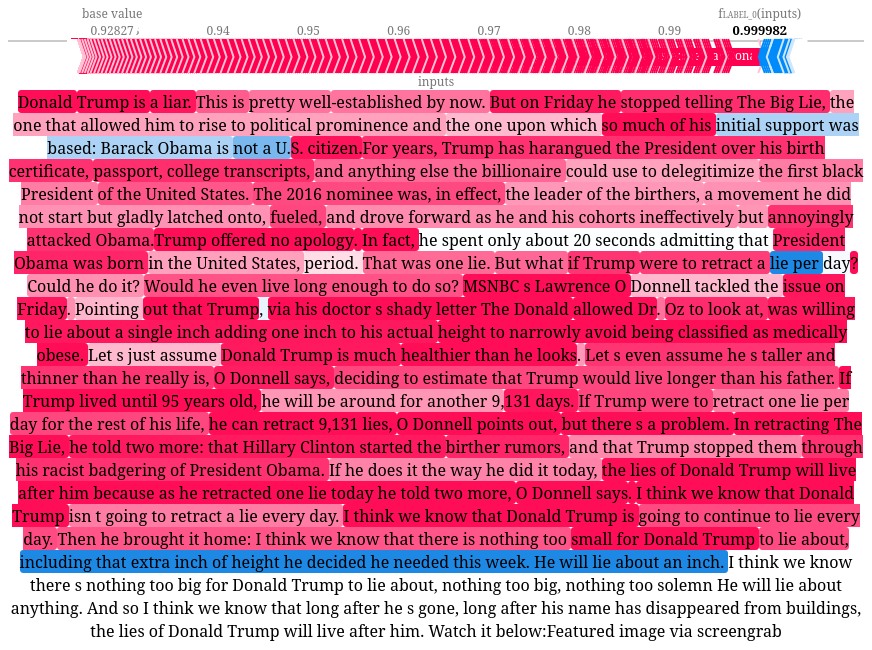
\includegraphics[scale=0.45]{FakeNewsExample2_forceplot.png}
    \caption[The explanation for the second fake news example.]{The explanation for the second fake news example. Observe that there are several coalitions between tokens such as "But on Friday he", "stopped telling The Big Lie" etc.}
    \label{fig:FakeNewsExample2_forceplot}
\end{figure}
\begin{figure}
    \centering
    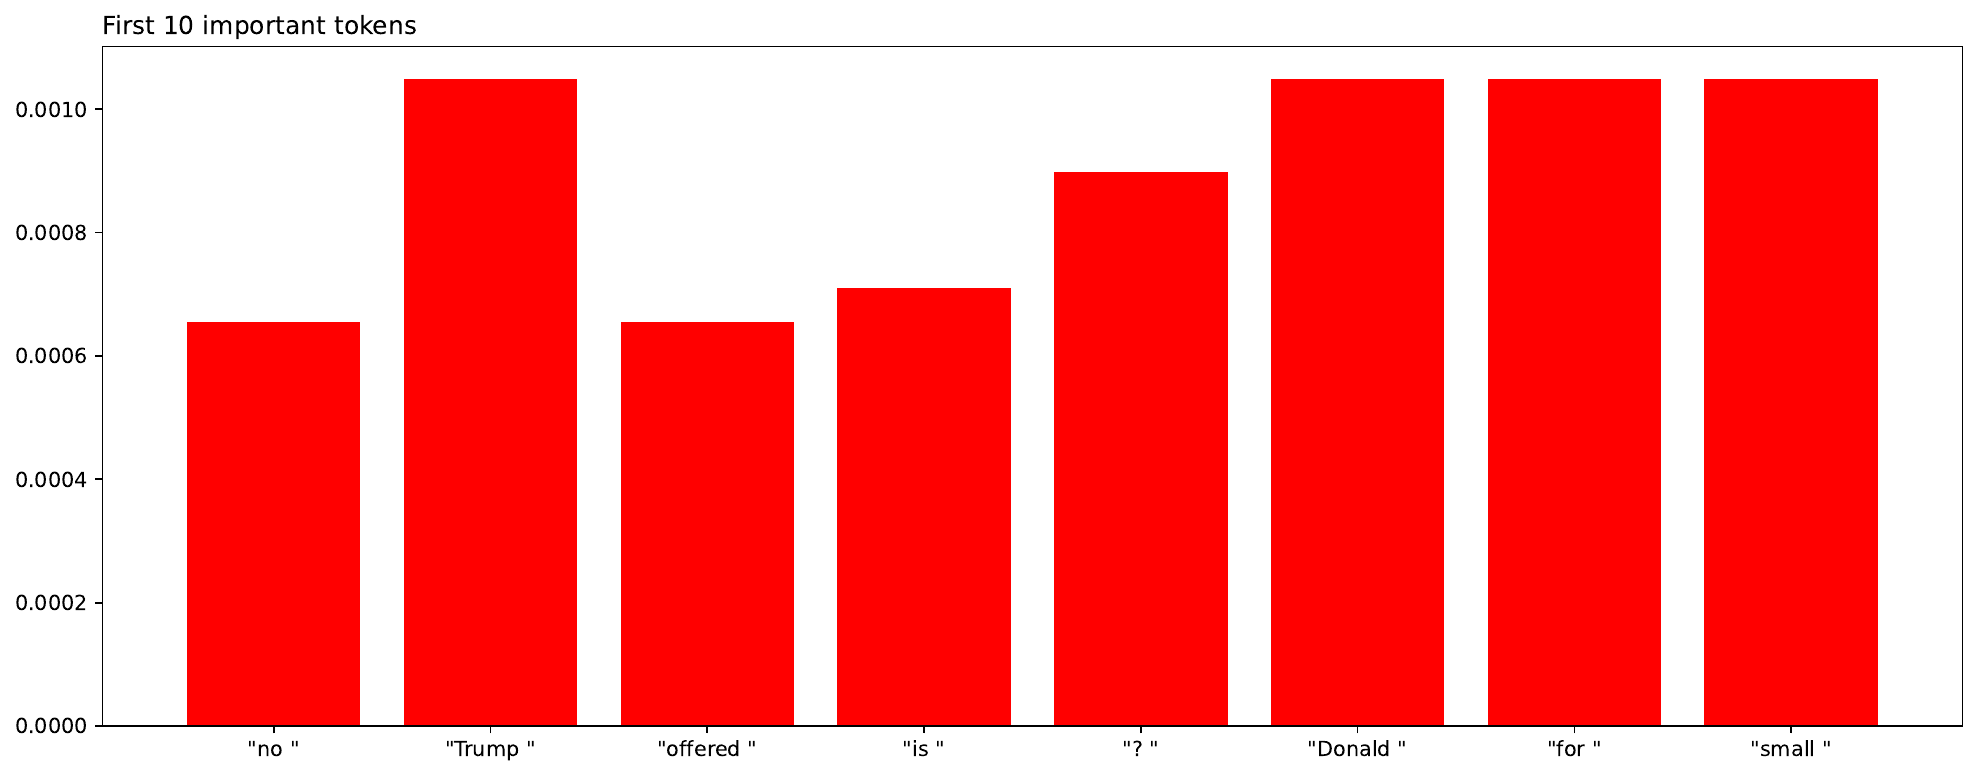
\includegraphics[scale=0.33]{FakeNewsExample2_barplot.png}
    \caption[The bar plot for the Owen values of the tokens in the second fake news example.]{The bar plot for the Owen values of the tokens in the second fake news example.  Since the news articles are long texts, we used a bar plot to visualize important tokens' Owen values.}
\end{figure}
We need to investigate why we obtain such high base values. Thus, to understand what the news content classifier thinks of the real news, we explain a real news instance from the train split. The example is shown in Fig.~\ref{fig:RealNewsExample1_forceplot}. We can easily see that the maximum share of Owen values go to three tokens: "(", "Reuters", ")". This suggests that the news content classifier has learned to distinguish news by source. In order to verify this intuition, we run one more real news example through the partition explainer. The explanation for the second example is illustrated in Fig.~\ref{fig:RealNewsExample2_forceplot}.\\
\begin{figure}
    \centering
    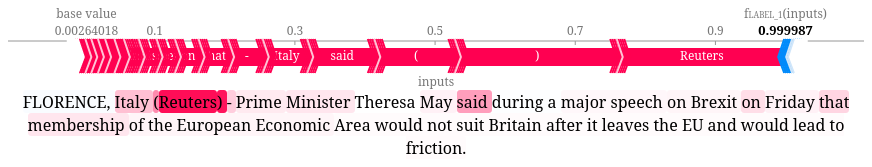
\includegraphics[scale=0.45]{RealNewsExample1_forceplot.png}
    \caption[The explanation for the first real news example.]{The explanation for the first real news example.}
    \label{fig:RealNewsExample1_forceplot}
\end{figure}
\begin{figure}
    \centering
    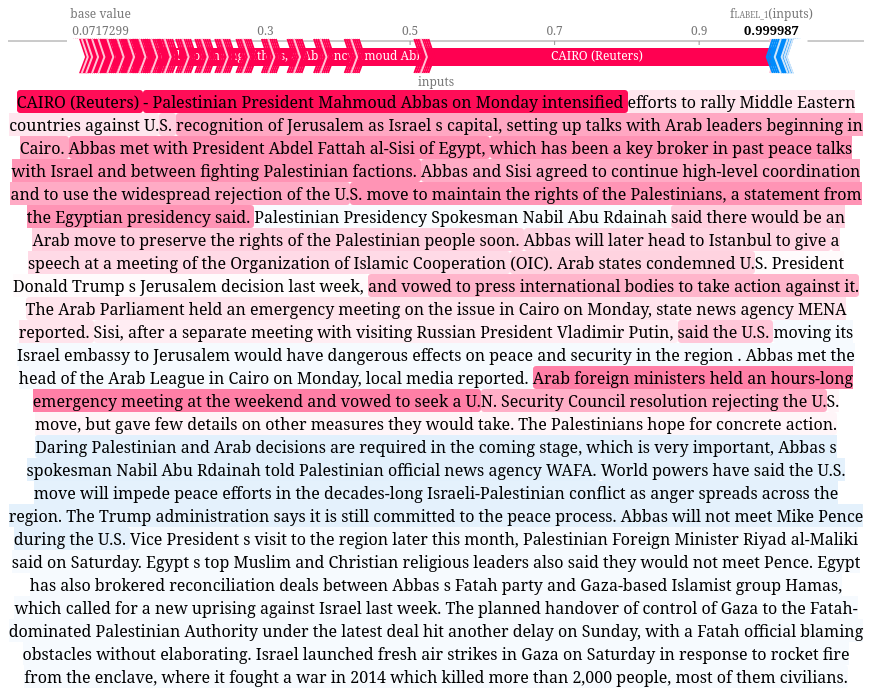
\includegraphics[scale=0.45]{RealNewsExample2_forceplot.png}
    \caption[The explanation for the second real news example.]{The explanation for the second real news example.}
    \label{fig:RealNewsExample2_forceplot}
\end{figure}
For the second example, we observe a coalition of tokens "CA", "IRO", " ", "(", "Reuters", ")". This coalition is given the highest Owen value of 0.48. The distribution of Owen values among tokens is illustrated in Fig.~\ref{fig:RealNewsExample2_barplot}. We can see that each token in the coalition was assigned almost equal Owen values. In two real news examples, the base value is really low. Again, one would expect around 0.5 for a binary classification setting.\\
\begin{figure}
    \centering
    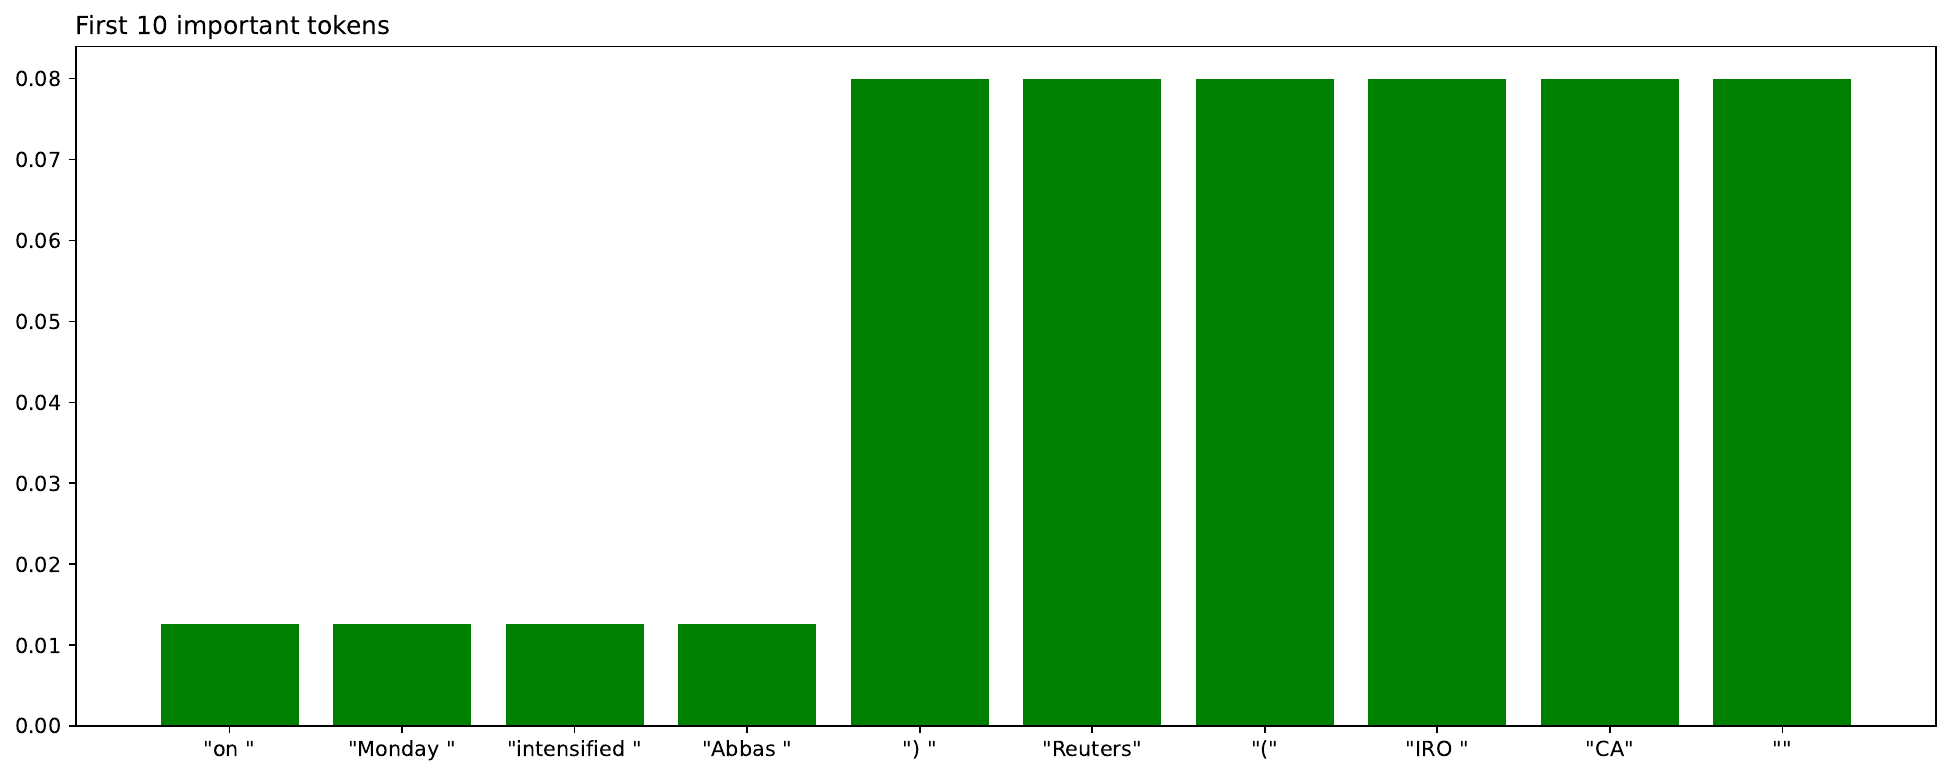
\includegraphics[scale=0.33]{RealNewsExample2_barplot.png}
    \caption[The bar plot of the 10 highest Owen values and their tokens for the second real news example.]{The bar plot of the 10 highest Owen values and their tokens for the second real news example.}
    \label{fig:RealNewsExample2_barplot}
\end{figure}
\textbf{Sensitivity Analysis.} Recall from~\ref{subsec:newContentModel_DatasetAndModel} that we reported that around 95\% of real news instances contained the text "(Reuters)". And also we expressed our concerns about the model basing most of its prediction on a couple of tokens. Now, let us consider that this model is deployed to detect fake news for a social platform. Once the adversaries realize this weakness of the model, then they could simply append "(Reuters)" to the beginning of their fake news and simply evade the detection. For a concrete example, see Fig.~\ref{fig:FakeNewsExample1Perturbed_forceplot}.\\
\begin{figure}
    \centering
    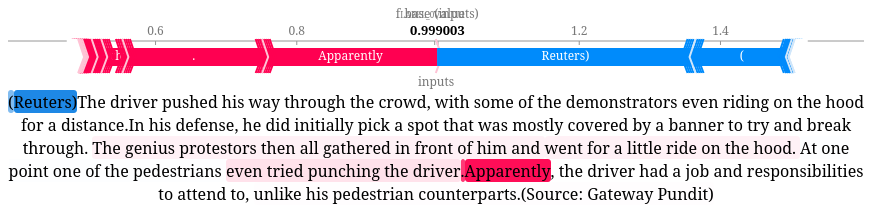
\includegraphics[scale=0.45]{FakeNewsExample1Perturbed_forceplot.png}
    \caption[The explanation for the perturbed first fake news instance.]{The explanation for the perturbed first fake news instance. This instance was predicted fake with more than 0.99 probability. We observe a very high base value as well. We see the negative effect of the token group "(Reuters)" on the force plot. Our intuition might be correct, however we might need a better alteration.}
    \label{fig:FakeNewsExample1Perturbed_forceplot}
\end{figure}
When we observe Fig.~\ref{fig:FakeNewsExample1Perturbed_forceplot}, we can easily see the adverse effect that the token "(" and the coalition "Reuters)" create is alleviated by assigning more Owen values to "Apparently" and ".". The model is still sure that this is a fake news instance. We might be required to adopt more complex adversarial approaches.\\
Knowing that the token group "(Reuters)" is never at the beginning of a real news article, we adopt more sophisticated changes in order to discover weaknesses of the model. We append a random string before "(Reuters)" and add the text " - " afterward, then append our fake news instance after this. This input sensitivity experiment shows that our intuition was correct for this instance. The explanation for this perturbation example is in Fig.~\ref{fig:FakeNewsExample1BetterPerturbed_forceplot}. We can observe that this fake news instance is now being predicted as real.\\
\begin{figure}
    \centering
    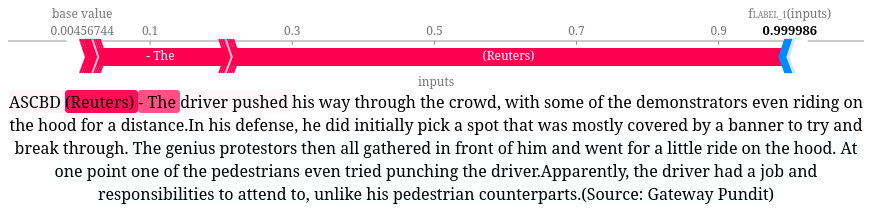
\includegraphics[scale=0.45]{FakeNewsExample1BetterPerturbed_forceplot.png}
    \caption[The explanation for the better perturbed first fake news instance.]{The explanation for the better perturbed first fake news instance. This instance was predicted real with over 0.99 probability. We can observe the dramatical probability change just by adding a couple words.}
    \label{fig:FakeNewsExample1BetterPerturbed_forceplot}
\end{figure}
\begin{figure}
    \centering
    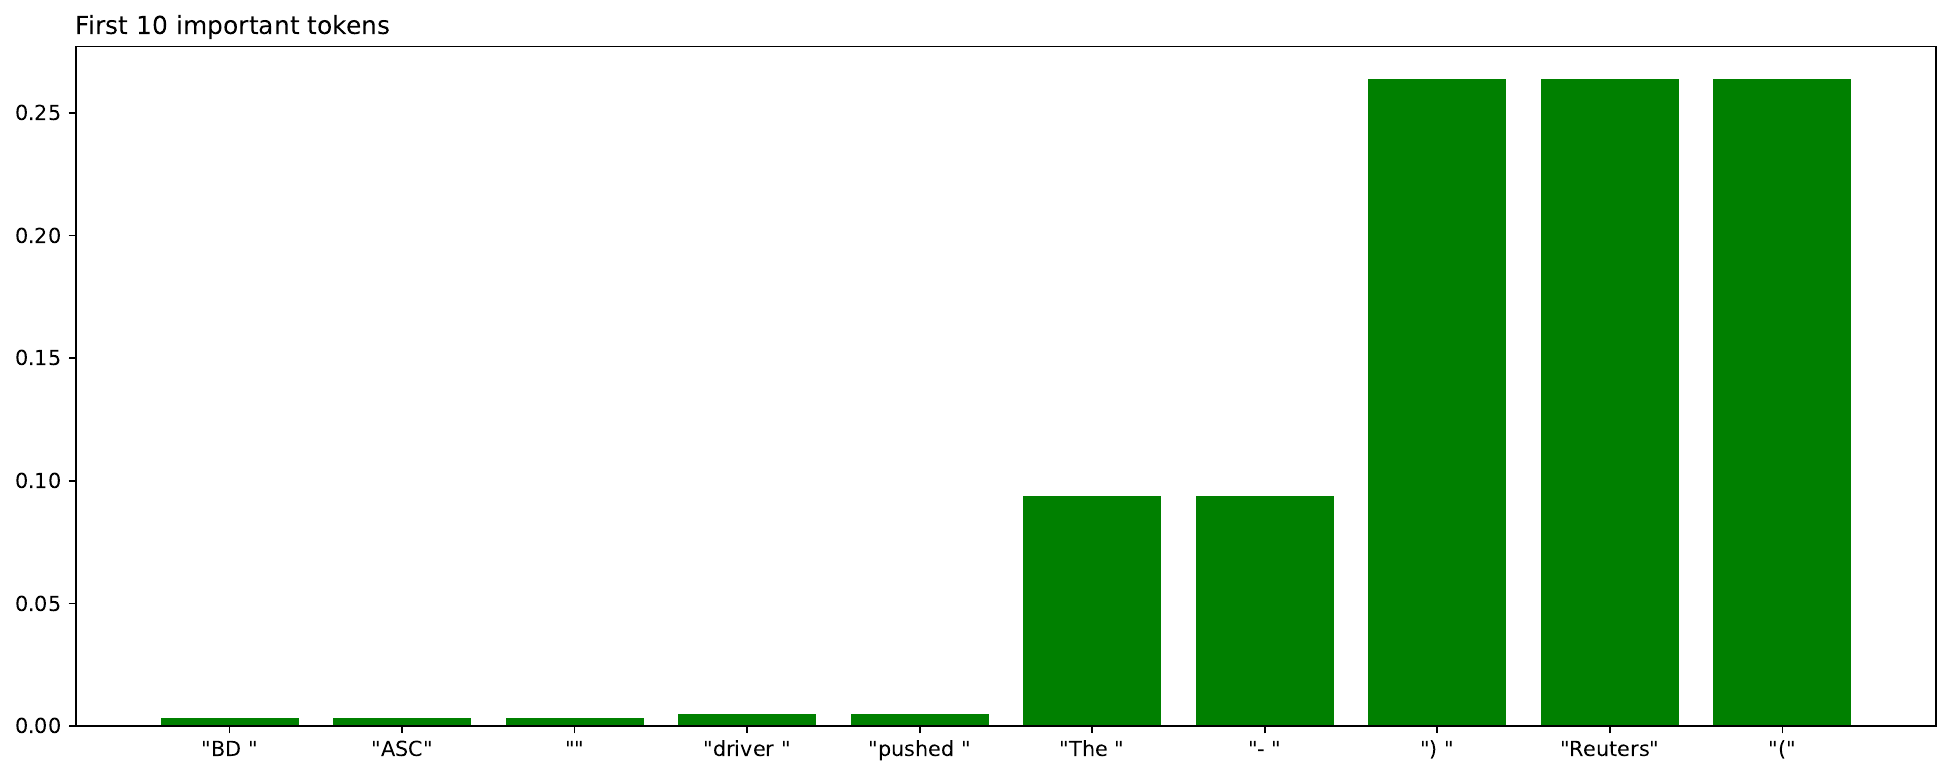
\includegraphics[scale=0.33]{FakeNewsExample1BetterPerturbed_barplot.png}
    \caption[The bar plot for the Owen values of better perturbed first fake news instance.]{The bar plot for the Owen values of better perturbed first fake news instance. Even a non-sense text like "ASCBD" is assigned one of the highest importance score.}
    \label{fig:FakeNewsExample1BetterPerturbed_barplot}
\end{figure}
\textbf{The Effect of The Model Architecture.} Now we can see the positional encodings' and attention mechanism's effect here. "ASCBD" is not a word, and it is tokenized as "ASC" and "BD" (can be seen in the x-axis of Fig.~\ref{fig:FakeNewsExample1BetterPerturbed_barplot}), with both tokens being assigned relatively large Owen values. Moreover, when the position of "(Reuters)" changes from the first to a later position, the model directly changes its mind. One more thing that comes to mind is the length of the text. Thus, we also applied the same technique to the second fake news example, whose feature relevance scores are better distributed. We got the same result for the second fake news example as well. We also observed similar behavior when explaining other training instances. We also tried using characters instead of character sequences and removing the space between "(Reuters)" and the initial character. The result was the same. This strongly suggests the model bases its predictions based on the existence and position of the token group "(Reuters)".\\
If we also consider the characteristics of DistilRoBERTa, we can see that the knowledge distillation process should be employed after the model is trained so that it can be deployed easily. Training a RoBERTa model with the cleaned dataset and then adopting the distillation process would be ideal. This way, more knowledge can be retained in the model.\\
We also conducted experiments with unseen data, but the results suggested the same outcome: clean the dataset and train again. Thus, we do not share the results from our unseen data experiment, as the results were parallel with the ones we have shared. In order to see the model's success without the existence of "(Reuters)" in real news, we need to train the news content classifier with the same hyperparameters in Table~\ref{tab:newsContentModelHyperparameters}, and the dataset should be changed such that the source part from the real news instances are removed, i.e., "$<location>$ (Reuters) -  $<newspiece>$" is changed to "$<newspiece>$" for real news.\\
We train the news content classifier by eliminating this issue from the dataset. We report the performance of the news content classifier in Table~\ref{tab:newsContentModelRetrainedPerformanceMetrics}.
\begin{table}
    \centering
    \begin{tabular}{c | c | c | c}
        \textbf{Accuracy} & \textbf{Precision} & \textbf{Recall} & \textbf{F1 score} \\
        \hline
        98.92\%           & 99.14\%            & 98.84\%         & 98.99\%           \\
    \end{tabular}
    \caption[The performance metrics for the retrained news content classifier.]{The performance metrics for the retrained news content classifier.}
    \label{tab:newsContentModelRetrainedPerformanceMetrics}
\end{table}
The performance stays the same, but let us inspect what the model has learned this time. To comparatively illustrate this, we ran the same examples we have introduced again and shared the force plot of the second fake news example in Fig.~\ref{fig:FakeNewsExample2_Retrained_forceplot}. Now that we have a lower base value for fake news, we can observe patterns caught by model in more depth. First, the high Owen values for the coalitions of contractions with the missing apostrophe, such as "MSNBC s", "doctor s", "Let s", "there s", "O Donnell" and "isn t" is the first pattern we observe in this instance. Second, full stops still get a relatively high Owen value. Moreover, even though the base value for fake news is decreased, it is still high.
\begin{figure}
    \centering
    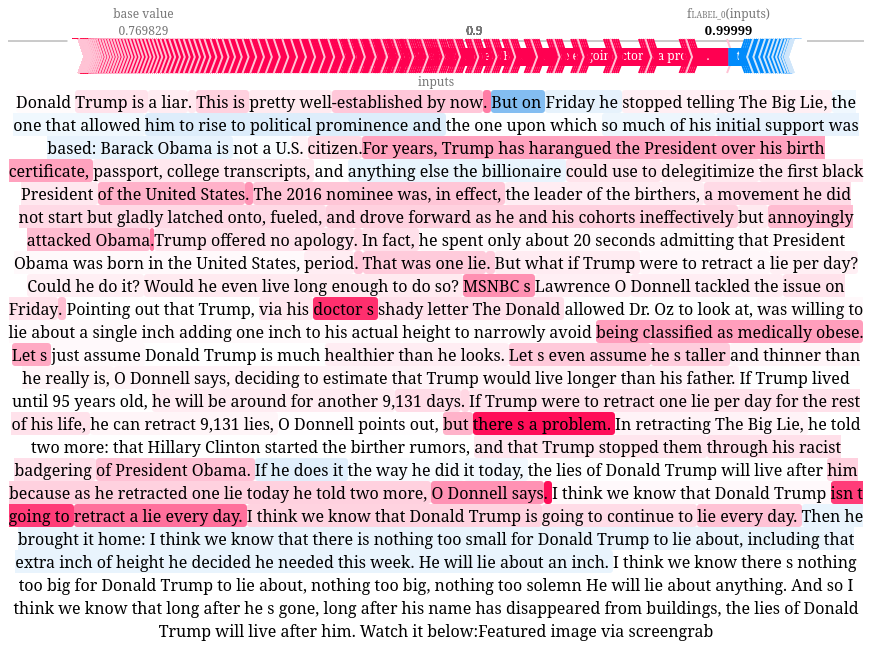
\includegraphics[scale=0.45]{FakeNewsExample2_Retrained_forceplot}
    \caption[The explanation of the second fake news instance for the retrained model.]{The explanation of the second fake news instance for the retrained model. Observe the lower base value and better distribution of Owen values.}
    \label{fig:FakeNewsExample2_Retrained_forceplot}
\end{figure}
To get a full understanding by comparing the explanation results, we also explain our second real news instance for our retrained model. The force plot of this explanation is shown in Fig.~\ref{fig:FakeNewsExample2_Retrained_forceplot}. We directly see the high base value, compared to Fig.~\ref{fig:RealNewsExample2_forceplot}, and also a better distribution of Owen values among the tokens and coalitions. The same detection for the lack of an apostrophe is also captured in this explanation. Coalitions like "Israel s", "Trump s", "Abbas s", "President s", and "Egypt s" have a large negative Owen value. This might suggest spelling mistakes such as leaving out the apostrophe are captured as informal by the news content classifier, even though these punctuations are removed in the tokenizer. There can be other reasons behind this behavior which can be uncovered by using explanation methods for other instances as well.
\begin{figure}
    \centering
    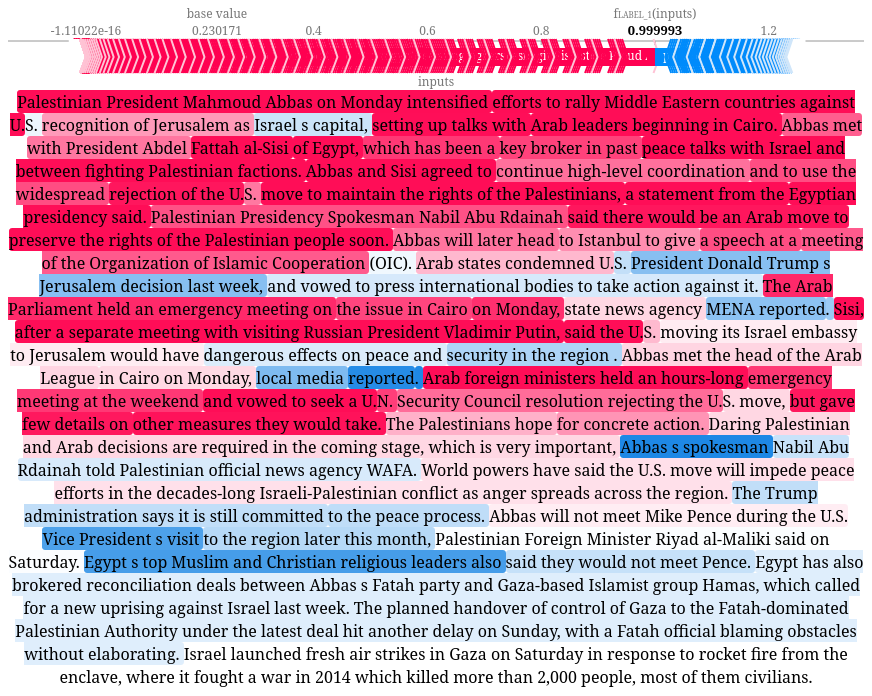
\includegraphics[scale=0.45]{RealNewsExample2_Retrained_forceplot}
    \caption[The explanation of the first fake news instance for the retrained model.]{The explanation of the first fake news instance for the retrained model. Observe the lower base value and better distribution of Owen values.}
    \label{fig:RealNewsExample2_Retrained_forceplot}
\end{figure}
We have seen that even though a model performs well, this doesn't mean that this model has learned the task. Since our news content classifier tries to distinguish between fake and real news using the patterns provided in the dataset, it is crucial to have a dataset that will not create the bias we observed. We used explanation techniques to uncover this issue with the news content classifier. We have seen the significance of adopting explanation methods to understand the behavior of the news content classifier. Thus, we have fulfilled \textbf{RO2} for news content classifiers.\\
Also, to fulfill \textbf{RO3} for this chapter, we report the understandability of the explanations provided by the partition explainer. Although we tried to explain long articles, the explanations were understandable, and the interactive behavior that allows viewing Owen values within coalitions helped us understand the impact of each token individually. With the help of bar plots, we were able to see the importance distribution between the first ten tokens. This allowed us to pinpoint the issue with the model even though it was performing very well. By utilizing simple visualization techniques, we were able to understand what the model had learned from the dataset. We used Python 3.7~\parencite{Python_Rossum}, PyTorch 1.11.0~\parencite{PyTorch_Paszke}, Transformers 4.19.2~\parencite{Transformers_Wolf}, SHAP 0.40.0~\parencite{AUnifiedApproach_Lundberg}, and Matplotlib 3.5.1~\parencite{Matplotlib_Hunter} for our implementations, visualizations, and experiments. The detailed usage of libraries, model explanation, and related work are provided in our GitHub repository\footnote{\url{https://github.com/sersery35/Explainability_of_FND_Models/tree/main/Huggingface}} \\
News content is highly related to the veracity of the news. Nonetheless, we might need more information to distinguish between fake and real news. In the next chapter, we introduce mixed approaches for FND in which we utilize news content data as well as social context data. Having this fusion of information proves to be very effective, as shown by~\citeauthor{UPFD_Dataset_Shu} (\citeyear{UPFD_Dataset_Shu}), models that use news content with social context are more successful than the models that utilize social context only.\\